\section{Аналитический раздел}

В данном разделе будет проведен анализ предметной области корпусов текстов.

\subsection{Анализ предметной области}

Корпусная лингвистика — это раздел компьютерной лингвистики, который занимается разработкой принципов построения и использования корпусов текстов с помощью компьютерных технологий.
Лингвистические корпуса представляют собой структурированные массивы данных, которые используются для изучения языковых единиц в текстах.
В рамках корпуса существует поисковая система, которая позволяет находить необходимые языковые единицы и примеры их употребления благодаря технологии текстовой разметки.
В свою очередь разметка может быть ручной и автоматической.~\cite{butenko2022}

\subsubsection*{Виды корпусов текстов}

В таблице \ref{tab:cc} приведена классификация корпусов текстов по разным признакам.

\begin{table}[H]
    \centering
    \begin{tabular}{|p{5cm}|p{11cm}|}
        \hline
        \textbf{Признак} & \textbf{Типы корпусов} \\ \hline
        Цель & Многоцелевые, специализированные \\ \hline
        Параллельность & Параллельные, сопоставимые \\ \hline
        % Тип языковых данных & Письменные, устные (речевые), смешанные \\ \hline
        % «Литературность» & Литературные, диалектные, разговорные, терминологические, смешанные \\ \hline
        % Жанр & Литературные, фольклорные, драматургические, публицистические \\ \hline
        % Назначение & Исследовательские, иллюстративные \\ \hline
        Динамичность & Динамические (мониторные), статические \\ \hline
        Разметка & Размеченные, неразмеченные \\ \hline
        Характер разметки & Морфологические, синтаксические, семантические, анафорические, просодические и т. д. \\ \hline
        % Доступность & Свободно доступные, коммерческие, закрытые \\ \hline
        Объем текстов & Полнотекстовые, «фрагментнотекстовые» \\ \hline
    \end{tabular}
    \caption{Классификация корпусов~\cite[с. 57]{cl2020}}
    \label{tab:cc}
\end{table}

Корпус технических текстов, для которого будет разрабатываться база данных в настоящей работе, является специализированным, параллельным, многоязыковым, динамическим (будет постоянно пополняться).

\subsubsection*{Параллельные корпусы}

Параллельные корпусы --- корпусы, представляющие собой множество текстов-оригиналов, написанных на каком-либо исходном языке, и текстов --- переводов этих исходных текстов на один или несколько других языков~\cite[с. 61]{cl2020}.

При подготовке параллельных корпусов и разработке программ для их обработки, требуется выровнять тексты --- установить соответствие между фрагментами текста оригинала и текста перевода.
Для решения этой задачи существуют различные методы автоматического выравнивания текстов по предложениям, грамматическим конструкциям, терминам, словам и словосочетаниям.~\cite[с. 61]{cl2020}

Ниже приведен пример выравнивания текстов на уровне предложений.

\begin{table}[H]
    \centering
    \begin{tabular}{|p{1cm}|p{7cm}|p{7cm}|}
        \hline
        1 & THE PLAY — for which Briony had designed the posters, programs and tickets, constructed the sales booth out of a folding screen tipped on its side, and lined the collection box in red crepe paper — was written by her in a two-day tempest of composition, causing her to miss a breakfast and a lunch. & Пьеса, для которой Брайони рисовала афиши, делала программки и билеты, сооружала из ширмы кассовую будку и обклеивала коробку для денежных сборов гофрированной красной бумагой, была написана ею за два дня в порыве вдохновения, заставлявшего ее забывать даже о еде. \\ \hline
        2 & When the preparations were complete, she had nothing to do but contemplate her finished draft and wait for the appearance of her cousins from the distant north. & Когда приготовления закончились, ей не оставалось ничего, кроме как созерцать свое творение и ждать появления кузенов и кузины, которые должны были прибыть с далекого севера. \\ \hline
    \end{tabular}
    \caption{Пример выравнивания текстов на уровне предложений~\cite[с. 62]{cl2020}}
    \label{tab:al}
\end{table}

\subsubsection*{Проблемы определения границ терминов}

При попытке проведения автоматического выравнивания на уровне терминов, возникает ряд проблем.
Среди них выделяют~\cite{butenko2022}:
\begin{itemize}
    \item неправильное определение границ терминов-словосочетаний, состоящих из двух и более слов и составных терминов; 
    \item  распознавание составных терминов и терминов-словосочетаний, состоящих из двух и более слов; в частности, распознавание лексической единицы как части составного термина или как свободной лексической единицы; 
    \item определение лексической единицы как термина в зависимости от контекста и тематики текста, в котором данная лексическая единица употребляется; 
    \item объемные списки терминов-кандидатов, которые необходимо проверять вручную, поскольку частота не является достаточным критерием для оценки того, является ли выделенное слово термином или нет. 
\end{itemize}

Точность определения границ термина при автоматической разметки является одной из основных лингвистических задач, а отсутствие на сегодняшний день веб-платформ для автоматической разметки русскоязычных текстов делает актуальным разработку таковой.

% \subsubsection{Тексты и разметки}

\subsubsection{Типы текстовых разметок}

Существует множество типов текстовых разметок.
Большинство современных корпусов относятся к корпусам морфологического или синтаксического вида~\cite[с. 56]{cl2020}.
% Таким, например, является НКРЯ --- Национальный Корпус Русского Языка~\cite{ruscorpora}.

Далее подробнее будут рассмотрены структурная и семантическая разметки, поскольку они являются основными типами разметки в параллельном корпусе технических текстов.
% TODO: экстралингвистическая разметка cl2020 c. 53

\newpage

\subsubsection*{Структурная разметка}

Структурная разметка предназначена для выделения структурных элементов текста (том, книга, часть, глава, действие, сноска, ремарка, стих, а также: абзац, предложение, словоформа и текстоформа --- таблица, формула и др.)~\cite{lesnikov2019}.
В контексте учебно-научных текстов структурная разметка использована для выделения названия статьи, авторов, оглавления, предисловия, введения и т.д.

На рисунке \ref{fig:ts} представлена структурная схема элементов учебно-научного текста. 

\begin{figure}[H]
	\centering
	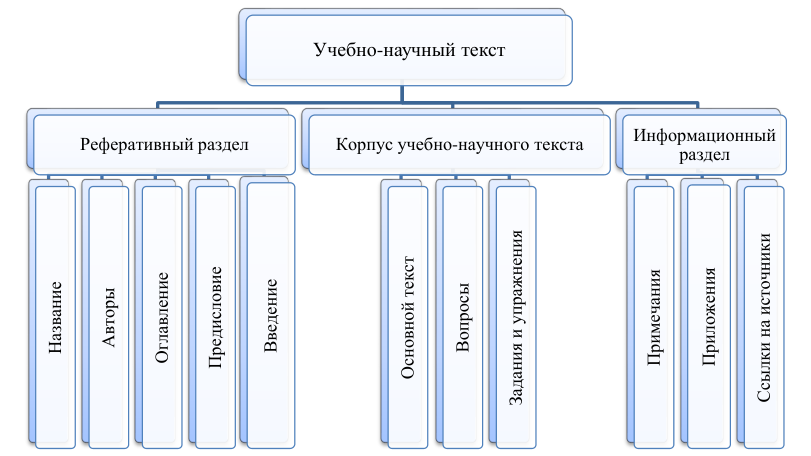
\includegraphics[width=0.9\textwidth]{img/tagging-struct.png}
	\caption{Структурные элементы учебно-научных текстов~\cite{butenko2021}}
	\label{fig:ts}
\end{figure}

\subsubsection*{Семантическая разметка}

Семантическая разметка помогает установить контекст высказывания и устранить двусмысленность. 
Основная цель семантической разметки --- <<формализировать>> значения слов и сделать тексты пригодными для машинной обработки.~\cite{butenko2022-2}

Существует множество видов семантических разметок.
Один из вариантов русской семантической разметки представлен на сайте Центра компьютерных и корпусных языковых исследований Ланкастерского университета~\cite[с. 51]{ucrel, cl2020}:

\begin{table}[H]
    \centering
    \begin{tabular}{|p{5cm}|p{11cm}|}
        \hline
        A & Общие понятия \\ \hline
        A1 & Общие понятия \\ \hline
        A1.1.1 & Обычные действия / Изголовление ч.-л. \\ \hline
        A1.1.1 & Повреждение и разрушение \\ \hline
        A1.2 & Пригодность \\ \hline
        A1.3 & Осторожность \\ \hline
        ... & ............................................................ \\ \hline
        B & Тело человека \\ \hline
        B1 & Анатомия и физиология \\ \hline
        B2 & Здоровье и болезнь \\ \hline
        ... & ............................................................ \\ \hline
        C & Искусства и ремесла \\ \hline
        ... & ............................................................ \\ \hline
    \end{tabular}
    \caption{Русская семантическая разметка~\cite{ucrel}}
    \label{tab:rsm}
\end{table}

В научно-технических текстах для семантической разметки могут использоваться семантические падежи Ч.~Филлмора~\cite{butenko2022-2}.

% \subsubsection*{Структура технических текстов}

\subsection{Существующие решения}

В современном мире существует множество параллельных корпусов (Opus, Linguee, MyMemory, Glosbe, Reverso, TAUS Data Cloud и др.)~\cite{butenko2020-1}, сервисов для автоматического выравнивания текстов (Hunalign, Euclid, Abbyy Aligner, Trados, Winalign, Wordfast tools, Giza++ и др.)~\cite[с. 62]{cl2020}, служб, позволяющих создавать собственные корпусы и производить в них поиск (SketchEngine~\cite{ske}, NoSketchEngine~\cite{noske}); инструментов для автоматического извлечения терминов (TerMine, TermExtraction, Terminology Extraction)~\cite{butenko2022} и прочих инструментов для работы с корпусами текстов (OpenCorpora~\cite{opencorpora}).

Но на данный момент не существует открытых параллельных корпусов технических текстов~\cite{butenko2020-2}.
Также нет открытых информационных систем, позволяющих одновременно производить разметку текста в параллельном корпусе, производить поиск по параллельному корпусу и организовать удобную работу множества разметчиков.

\subsection{Формализация задачи}

В ходе выполнения курсовой работы необходимо спроектировать и разработать базу данных для хранения документов --- технических текстов на разных языках, их разметок, и информации о пользователях базы данных.

Для взаимодействия с базой данных необходимо разработать интерфейс, предоставляющий возможности
\begin{itemize}
    \item добавления новых документов в базу данных,
    \item добавления новых разметок в базу данных,
    \item произведения поиска по текстам и разметкам, хранящимся в базе данных.
\end{itemize}

\subsection{Формализация данных}

Разрабатываемая база данных должна хранить информацию о следующих сущностях:
\begin{itemize}
    \item пользователь;
    \item документ;
    \item метаданные о документе --- автор;
    \item задание на разметку;
    \item структурная разметка;
    \item терминологическая разметка.
\end{itemize}

% \subsection{Сущности базы данных}

% ERD в нотации Чена

\begin{figure}[H]
	\centering
	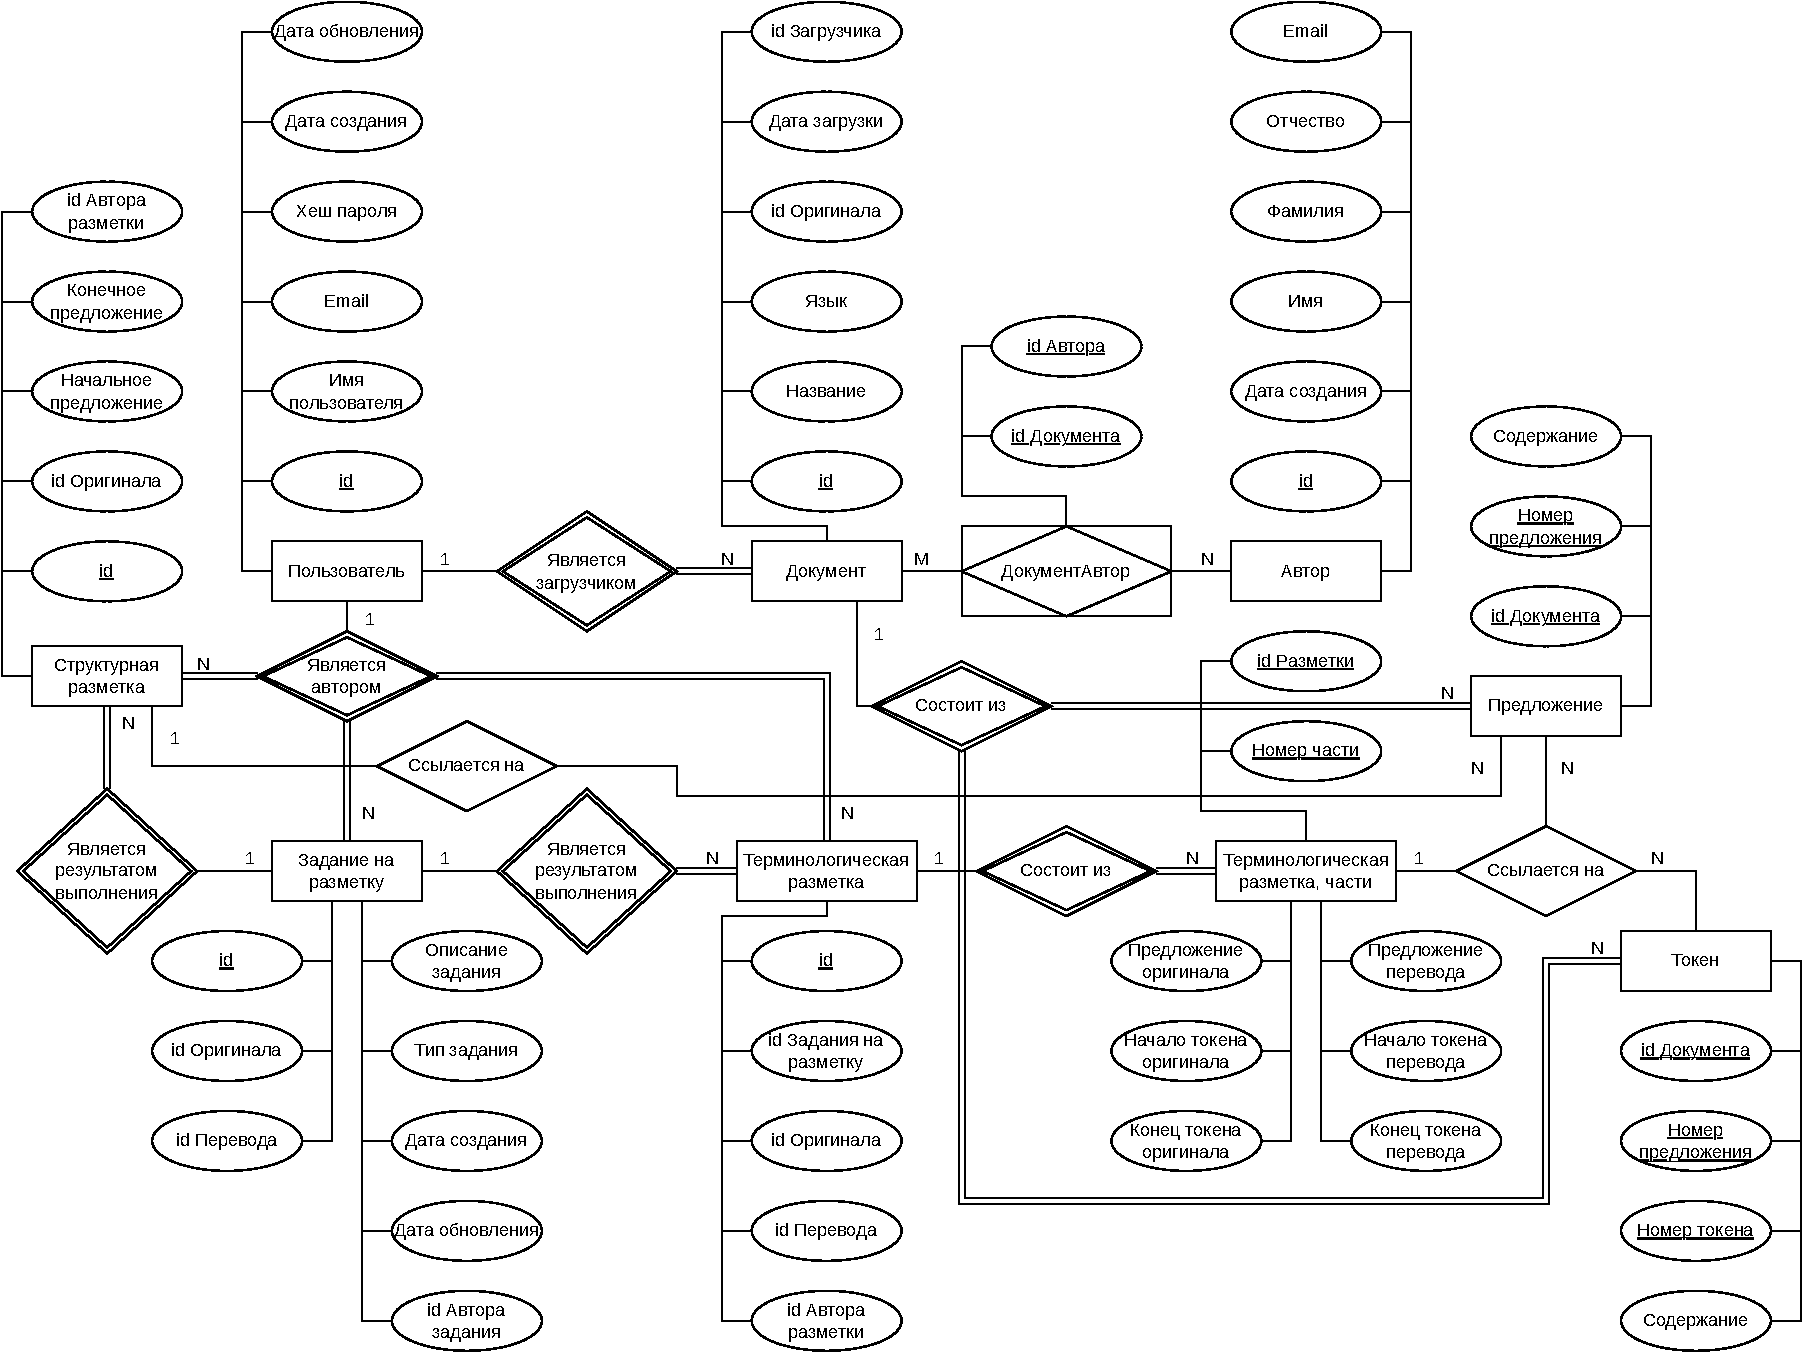
\includegraphics[angle=90, width=\textwidth]{diag/chen-v4.pdf}
	\caption{ER-диаграмма в нотации Чена}
	\label{fig:chen}
\end{figure}

\subsection{Формализация и описание пользователей}

\subsection{Сценарии использования}

% Use-Case диаграмма

\subsection{Анализ существующих баз данных}

\subsubsection{Выбор базы данных}

\subsection{Вывод}
